



%----------------------------------------------------------------------------------------

\newpage


%\section[Existing Models][Modèles existants]{Existing Models}{Modèles existants}
\section{Exploring macroscopic models of co-evolution}{Explorer les modèles macroscopiques de co-évolution}

\label{sec:macrocoevolexplo}

%----------------------------------------------------------------------------------------



\bpar{
We first propose to introduce co-evolution models at the macroscopic scale by exploring the results produced by an existing model, what will also allow to introduce methods and indicators that are necessary to the exploration, and to grasp the typical questions linked to this type of models. In particular, we proceed to a systematic exploration of the SimpopNet model \cite{schmitt2014modelisation}, which is to the best of our knowledge one of the rare initiatives to model co-evolution within a system of cities.
}{
Nous proposons dans un premier temps d'introduire les modèles de co-évolution à l'échelle macroscopique en explorant les résultats produits par un modèle existant, ce qui permettra également d'introduire les méthodes et indicateurs nécessaires à l'exploration, ainsi que d'appréhender les questionnements typiques liés à ce type de modèles. En particulier, nous procédons à une exploration systématique du modèle SimpopNet~\cite{schmitt2014modelisation}, à notre connaissance l'une des rares initiatives pour modéliser la co-évolution au sein d'un système de villes.
}



%%%%%%%%%%%%%%%%%%%%%%%
\subsection{Context}{Contexte}


\bpar{
A considerable gain in knowledge can be observed, from the conceptual or thematic description of a model, to its mathematical formalisation, its implementation, its systematic exploration, up to its exploration in deep with the help of specific meta-heuristics. Our postulate, that is a consequence of both our positioning (see \autoref{ch:positioning} on simulation) and experiments of which previously developed models are part, is that it is important, but furthermore of a \emph{qualitative} nature, in the sense that the nature of knowledge follows abrupt transitions during the advance of the investigation in this continuum.
}{
Un gain considérable de connaissances peut s'observer, de la description conceptuelle ou thématique d'un modèle, à sa formalisation mathématique, son implémentation, son exploration systématique, jusqu'à son exploration approfondie à l'aide de méta-heuristiques spécifiques. Notre postulat, qui découle à la fois de notre positionnement (voir le chapitre~\ref{ch:positioning} sur la simulation) et d'expériences dont les modèles déroulés précédemment font partie, est que celui-ci est important, mais surtout de nature \emph{qualitative}, c'est-à-dire que la nature même des connaissances subit des transitions abruptes lors de l'avancée de la démarche dans ce continuum.
}


\bpar{
The SimpopNet model introduced by~\cite{schmitt2014modelisation}, which is to our knowledge the only co-evolution model in the perspective of the evolutive urban theory. Its behavior was however not systematically explored, what makes it a good candidate for our approach.
}{
Le modèle SimpopNet introduit par~\cite{schmitt2014modelisation}, est à notre connaissance l'unique modèle de co-évolution selon la perspective de la théorie évolutive des villes. Son comportement n'a cependant pas été exploré systématiquement, ce qui en fait un bon candidat pour notre démarche.
}

\subsubsection{Studied model}{Modèle étudié}


\bpar{
We briefly reformulate the model, following the notations for the formalization of the interaction model in~\ref{sec:interactiongibrat}, since a certain number of parameters and processes are similar. Cities grow following a specification that rejoins equation~\ref{eq:interactiongibrat:model}, i.e. in this specific case
}{
Nous reformulons brièvement le modèle, suivant les notations de la formulation du modèle d'interaction en~\ref{sec:interactiongibrat}, un certain nombre de paramètres et de processus se recoupant. Les villes croissent suivant une spécification qui peut être rapprochée de l'équation~\ref{eq:interactiongibrat:model}, c'est-à-dire dans ce cas spécifique
}
\[
\mu_i(t+1) - \mu_i (t) = \mu_i (t) \cdot \frac{\lambda^{\beta}}{N} \sum_{j} \frac{V_{ij}}{<V_{ij}>}
\]
\bpar{
where the potential is of the form $V_{ij} = \mu_j / d_{ij}^\beta$ and $V_{ii}=0$, and $\beta$ is a parameter for the distance decay and $\lambda$ shape parameter for the decay function. We thus find our formulation, with $r_0 = 0$ and $w_G = \lambda^\beta \cdot N$. Since $\lambda$ gives the typical distance of interaction, it will be noted $d_G$ in the following, and $\beta$ will be noted $\gamma_G$ (it is indeed a level of hierarchy as a function of distance).
}{
où le potentiel est de la forme $V_{ij} = \mu_j / d_{ij}^\beta$ et $V_{ii}=0$, et $\beta$ est un paramètre de vitesse de décroissance en fonction de la distance et $\lambda$ paramètre de forme de la fonction de décroissance. Nous retrouvons ainsi notre formulation, avec $r_0 = 0$ et $w_G = \lambda^\beta \cdot N$. Comme $\lambda$ fixe la distance typique d'interaction, nous le noterons par la suite $d_G$, et $\beta$ sera noté $\gamma_G$ (il s'agit bien d'un niveau de hiérarchie en fonction de la distance).
}

%Le potentiel d'interaction ne dépend pas de la population de la ville d'origine, et le choix d'une fonction puissance permet de combiner un paramètre de décroissance $\lambda$ à un paramètre de forme $\beta$.

\bpar{
The network growths at each time step through a process that can be seen as a potential breakdown (as described in chapter~\ref{ch:thematic}): a couple of cities is chosen, the first according to populations with a hierarchy $\gamma_N$ (i.e. with a probability proportional to ${\mu_i}^{\gamma_N}$) and the second following interaction forces $\mu_i \mu_j / d_{ij}^\beta$ with the same hierarchy $\gamma_N$. A link is then created if the network is not efficient enough, i.e. if $d_{ij}/d^{(N)}_{ij}> \theta_N$. The links created at a date $t$ have a speed $v(t)$, which will depend on current transportation technologies. The creation of new intersections to yield a planar graph is only done for links with a similar speed.
}{
Le réseau croît à chaque pas de temps par un processus que nous pouvons qualifier de rupture de potentiel (comme décrit au chapitre~\ref{ch:thematic}) : un couple de villes est choisi, la première selon les populations avec une hiérarchie $\gamma_N$ (c'est-à-dire avec une probabilité proportionnelle à ${\mu_i}^{\gamma_N}$) et la seconde selon les forces d'interactions $\mu_i \mu_j / d_{ij}^\beta$ avec la même hiérarchie $\gamma_N$. Un lien est alors créé si le réseau n'est pas assez efficace, c'est-à-dire si $d_{ij}/d^{(N)}_{ij}> \theta_N$. Les liens créés à une date $t$ ont une vitesse $v(t)$, qui dépendra des technologies de transport courantes. La création de nouvelles intersections pour produire un graphe planaire n'est effectuée que pour les liens de vitesse semblable.
}

\bpar{
In order to study a stylized version of the model, we consider a configuration such that $v(t > 0) = v_0$ and $v(0) = 1$ (the initial model considers three values for speed that correspond to the reality of transportation technologies between 1830 and 2000).
}{
Afin d'étudier une version stylisée du modèle, nous considérons une configuration telle que $v(t > 0) = v_0$ et $v(0) = 1$ (le modèle initial considère trois valeurs de la vitesse correspondant aux réalités des technologies de transport entre 1830 et 2000).
}


\subsubsection{Perspectives}{Perspectives}

\bpar{
We can put the structure of this model into perspective. Some modeling choices are not in direct consistency with the application it is used for: for example, such a precision in the parametrization of dates and speeds (historical dates from 1800 to 2000 and speed that approximatively corresponds to transportation technologies) makes it a hybrid model, and should correspond to an application on a real spatial configuration. In a synthetic configuration as used in the model, these parameters have a sense only if we know the behavior of simulated dynamics, and in particular the role of the spatial configuration, i.e. if we are able to differentiate effects linked to the dynamics from effects linked to the initial spatial configuration.
}{
Mettons en perspective la structure de ce modèle. Certains choix de modélisation ne sont pas en cohérence directe avec l'application qui en est faite : par exemple, une telle précision dans la paramétrisation des dates et des vitesses (dates historiques de 1800 à 2000 et vitesse correspondant approximativement aux technologiques de transport) en fait un modèle hybride, et devrait correspondre à une application sur une configuration spatiale réelle. Dans une configuration synthétique comme employée dans le modèle, ces paramètres n'ont de sens que si l'on connait le comportement des dynamiques simulées, et en particulier le rôle de la configuration spatiale, c'est-à-dire si l'on est capable de différencier effets liés à la dynamique et effets liés à la configuration spatiale initiale. 
}

\bpar{
Furthermore, the use of the interaction model without the endogenous Gibrat term would be difficultly adaptable to an application of the model on real data since the values we obtained in the precedent studies of interaction models, but stays relevant in a stylized model, in order to understand the interaction processes in an isolated way, as we will do later (keeping in mind that this knowledge does not necessarily describes the coupled behavior, since the interaction between processes can lead to the emergence of new behaviors).
}{
D'autre part, l'utilisation du modèle d'interaction sans le terme de Gibrat endogène serait difficilement adaptable pour une application du modèle sur données réelles vu les valeurs obtenues dans les études précédentes des modèles d'interaction, mais est bien cohérent dans un modèle stylisé, afin de comprendre les processus d'interaction de manière isolée, comme nous le ferons plus loin (tout en gardant à l'esprit que cette connaissance ne reflète pas nécessairement le comportement couplé, l'interaction entre les processus pouvant faire émerger de nouveaux comportements).
}





\bpar{
The formulation of the potential, given above, as $(\lambda / d_{ij})^\beta$, implies that $\lambda$ captures both the weight of the potential and the shape of the decreasing function, but imposes a dependence between these two effects, on the contrary to the specification we use previously. It furthermore does not allow an interpretation in terms of limit flows\footnote{The weight parameter in our model in~\ref{sec:interactiongibrat} gives indeed the value of the flow when the distance attenuation goes to infinity and for all the population.}.
}{
La formulation du potentiel, donnée ci-dessus, en $(\lambda / d_{ij})^\beta$, implique que $\lambda$ capture à la fois le poids du potentiel et la forme de la décroissance, mais contraint à une dépendance entre ces deux effets, contrairement à la spécification que nous avons utilisé précédemment. Elle ne permet par ailleurs pas d'interprétation en terme de flux limite\footnote{Le paramètre de poids dans notre modèle en~\ref{sec:interactiongibrat} donne en fait la valeur du flux lorsque l'atténuation par la distance tend vers l'infini et pour l'ensemble de la population.}.
}


\bpar{
Finally, rules allowing variable values for $v(t)$ and the non-planarity mechanism\footnote{When a new link is constructed, it does create intersections only with links of similar speed.}, allows the introduction of a tunnel effect, which is as we recall is the absence of interaction of an infrastructure traversing a territory with it. The effect is however exogenous since explicitly specified in model rules, on the contrary to the interaction model with feedback of flows, in which the variations of $w_N$ and $d_N$ should capture an endogenous tunnel effect. The introduction of specific indicators to measure it would be an interesting development direction, but we stay here at considering the hierarchy of centralities which is already a good indicator for it\footnote{Indeed, a highly hierarchical distribution of accessibilities means that there exists a small number of cities very accessible and a large number with a low accessibility. If main cities reasonably cover the space, then their links necessarily ignore the overflown cities with low accessibility, otherwise the distribution would be less hierarchical.}.
}{
Enfin, les règles permettant des valeurs variables de $v(t)$ et le mécanisme de non-planarité du réseau\footnote{Lorsqu'un nouveau lien est construit, celui-ci ne forme des intersections qu'avec les liens de vitesse similaire.}, permet l'introduction d'un effet tunnel, qui nous le rappelons est la non-interaction d'une infrastructure traversant un territoire avec celui-ci. L'effet est cependant exogène puisque spécifié explicitement dans les règles du modèle, contrairement au modèle d'interaction avec rétroaction des flux, dans lequel les variations de $w_N$ et $d_N$ doivent capturer un effet tunnel endogène. L'introduction d'indicateurs spécifiques pour le mesurer serait une piste intéressante de développement, mais nous nous contentons de regarder ici la hiérarchie des centralités qui en est déjà un bon indicateur\footnote{En effet, une distribution très hiérarchique des accessibilités signifie qu'il existe un petit nombre de villes très accessibles et un grand nombre peu accessibles. Si les villes importantes couvrent raisonnablement l'espace, alors leurs liens ignorent nécessairement les villes peu accessibles survolées, sinon la distribution serait moins hiérarchique.}.
}

% rq : this last argument works but is rather subtle to grasp ! illsutrate with a toy model ?


%%%%%%%%%%%%%%%%%%%%%%%
\subsection{Methodology}{Méthode}

\subsubsection{Spatial configuration}{Configuration spatiale}


\bpar{
An important aspect for understanding co-evolution processes implied in this model is the role of the initial spatial configuration in emerging patterns observed. We therefore apply the methodology developed in~\ref{sec:computation}, which allows to extend the sensitivity analysis of a model to spatial meta-parameters\footnote{We recall that in our case a meta-parameter is a parameter allowing to generate an initial configuration upstream of the model.}.
}{
Un aspect important de la compréhension des processus de co-évolution impliqués dans ce modèle est le rôle de la configuration spatiale initiale dans les motifs émergents observés. Nous appliquons pour cela la méthodologie développée en~\ref{sec:computation}, qui permet d'étendre l'analyse de sensibilité d'un modèle à des méta-paramètres spatiaux\footnote{Nous rappelons que dans notre cas un méta-paramètre est un paramètre permettant de générer une configuration initiale en amont du modèle.}.
}


\paragraph{Generation of synthetic configurations}{Génération de configurations synthétiques}

\bpar{
A synthetic system of cities is constructed the following way (see Appendix~\ref{app:sec:syntheticdata} for the notion of synthetic data, calibrated at the first and the second order). A fixed number $N$ of cities is uniformly distributed in space, under the constraint of a minimal distance between each, and their population is attributed following a rank-size law which parameters $P_{m}$ and $\alpha$ can be adjusted (the distribution of city sizes in the initial model corresponds to $\alpha\simeq 0.68$ with $R^2=0.98$).
}{
Une système de villes synthétique est construit de la façon suivante (voir l'Annexe~\ref{app:sec:syntheticdata} pour la notion de données synthétiques, calibrées au premier et second ordre). Un nombre fixé de villes $N$ est réparti uniformément dans l'espace en respectant une distance minimale entre chaque, et leur population est attribuée suivant une loi rang-taille dont les paramètres $P_{m}$ et $\alpha$ peuvent être ajustés (la distribution de la taille des villes dans le modèle initial correspond à $\alpha\simeq 0.68$ avec $R^2=0.98$).
}


\bpar{
A skeleton of network is created by progressive connection: the algorithm connects cities two by two by closest neighbour in terms of euclidian distance, and then iteratively selects randomly a cluster and connects it perpendicularly to the closest link outside the cluster. The network is then extended by the creation of local shortcuts, through a repetition $n_s$ times of the random selection of a city according to populations, and its connection to a neighbour in a radius $r_s$ under conditions of a maximal degree $d_s$. The final network is then made planar.
}{
Un squelette de réseau est créé par connection progressive : l'algorithme connecte les villes deux à deux par plus proche voisin en distance euclidienne, puis itérativement sélectionne un cluster aléatoirement et le connecte perpendiculairement au lien le plus proche hors du cluster. Le réseau est ensuite étoffé par la création de raccourcis locaux, par répétitions $n_s$ fois de la sélection aléatoire d'une ville selon les populations, et sa connexion à un voisin dans un rayon $r_s$ sous conditions de degré maximal $d_s$. Le réseau final est ensuite planarisé.
}


\bpar{
This process creates networks that visually correspond (in terms of the order of magnitude of the number of loops, and their spatial range) to the initialization of the model, knowing that a single instance of the network does not allow to determine distributions of topological parameters for which a more precise calibration could be done.
}{
Cette procédure crée des réseaux correspondant visuellement (ordre de grandeur du nombre de boucles, portée spatiale de celles-ci) à l'initialisation du modèle, sachant qu'une instance du réseau ne permet pas de déterminer les distributions de paramètres topologiques sur lesquels une calibration plus fine pourrait être opérée.
}


\subsubsection{Indicators}{Indicateurs}


\bpar{
A crucial aspect of the study of simulation models is the definition of relevant indicators, particularly in the case of synthetic models where it is not possible to produce outputs that are directly linked to data for example. Very general stylized facts, as aiming at producing an urban hierarchy or a network hierarchy, are relatively limited. Moreover, the hierarchy is mechanically produced by most models including aggregation processes. We therefore need more elaborated indicators to understand the dynamics of the system. These indicators must in particular give elements of answer to the following questions:
\begin{itemize}
	\item types of systems of cities produced by the model;
	\item change in time of the organization of the system of cities;
	\item typical profiles of trajectories;
	\item ability to ``produce some co-evolution''.
\end{itemize}
}{
Un aspect crucial de l'étude des modèles de simulation est la définition d'indicateurs pertinents, surtout dans le cas de modèles synthétiques où il n'est pas possible de produire des sorties directement liées aux données par exemple. Des faits stylisés très généraux, comme vouloir produire une hiérarchie urbaine ou une hiérarchie de réseau, sont relativement limités. De plus, la hiérarchie est produite mécaniquement par la majorité des modèles incluant des processus d'agrégation. Il faut donc des indicateurs plus élaborés pour comprendre les dynamiques du système. Ces indicateurs doivent notamment apporter des éléments de réponse aux questions suivantes : 
 \begin{itemize}
 	\item types de systèmes de villes produits par le modèle ;
 	\item changement dans le temps de l'organisation du système de ville ;
 	\item profils typiques de trajectoires ;
 	\item capacité à ``produire de la co-évolution''.
 \end{itemize}
}


\bpar{
In order to concentrate on the ability of the model to produce trajectories that are both diverse and complex, and for example its ability to produce bifurcations that would manifest as inversions in ranks, and also its ability to capture different aspects of co-evolutive dynamics, we propose a set of indicators, including for example lagged correlation measures in the spirit of causality regimes exhibited in~\ref{sec:causalityregimes}, or a correlation measure as a function of distance, to understand the role of spatial interactions in the coupling of trajectories. Given a variable $X_i(t)$ defined for each city and in time (that will be the population or centrality measures for example), we define the following indicators.
}{
Pour se concentrer sur la capacité du modèle à produire des trajectoires à la fois diverses et complexes, et par exemple sa capacité à produire des bifurcations qui se traduiraient par inversions de rang, ainsi que sa capacité à capturer différents aspects des dynamiques co-évolutives, nous proposons un jeu d'indicateurs, incluant par exemple des mesures de corrélation retardée en écho aux régimes de causalité exhibés en~\ref{sec:causalityregimes}, ou une mesure de corrélation en fonction de la distance, pour comprendre le rôle des interactions spatiales dans les couplages de trajectoires. Étant donné une variable $X_i(t)$ définie sur chacune des villes et dans le temps (qui pourra être la population ou des mesures de centralité par exemple), nous définissons les indicateurs suivants.
}


\bpar{
\begin{itemize}
	\item Indicators characterizing the distribution of $X_i$ in time: hierarchy (slope of the least squares adjustment of $X_i$ as a function of rank) $\alpha (t)$, entropy of the distribution $\varepsilon (t)$, descriptive statistics (average $\hat{\Eb{X}} (t)$ and standard deviation $\hat{\sigma} (t)$).
	\item Rank correlation between the initial time and the final time, which translates the quantity of change in the hierarchy during the evolution of the system, and is defined by $\rho_r = \hat{\rho}\left[rg(X_i(t=0)),rg(X_i(t=t_f))\right]$, where $rg(X_i)$ is the rank of $X_i$ among all values.
	\item Diversity of trajectories $\mathcal{D}\left[X_i\right]$, which captures a diversity of time series profiles for the considered variable. With $\tilde{X}_i(t)\in \left[0;1\right]$ the trajectories that have been individually rescaled, it is defined by
\[
\mathcal{D}\left[X_i\right] = \frac{2}{N\cdot(N-1)}\sum_{i<j} \left(\frac{1}{T}\int_{t} \left(\tilde{X}_i(t) - \tilde{X}_j(t)\right)^2 \right)^{\frac{1}{2}}
\]
	\item Changes in direction of trajectories $\mathcal{C}\left[X_i\right]$, that we take as the number of inflexion points. In the context of such a type of model, which mainly produces monotonous trajectories, this indicator witnesses in a certain way of a ``complexity'' of trajectories.
	\item Correlations as a function of distance, to understand the way the effect of distance is translated at the macroscopic scale. The profile of this function, regarding interaction distance parameters included in the model, will translate the tendency of the model to lead to the emergence of one level of interaction or the other. It is computed as
\[
\rho_d = \hat{\rho}\left[(X(\vec{x}_k,Y(\vec{x}_{k'}))\right]
\]
where $X_i, Y_i$ are the two variables considered and $(k,k')$ the set of couples such that $\norm{\vec{x}_k-\vec{x}_{k'}} - d \leq \varepsilon$ with $\varepsilon$ a tolerance threshold (in practice taken to regroup couples by distance deciles).
	\item Lagged correlations between the variations of variables, to identify causality patterns between variables $X$ and $Y$. The patterns $\hat{\rho}_{\tau}$ for all variables, and for $\tau$ lag or anticipation, must be understood in the sense of potential regimes, explored in~\ref{sec:causalityregimes}.
\[
\rho_{\tau} = \hat{\rho}\left[\Delta X(t-\tau),\Delta Y(t)\right]
\]
\end{itemize}
}{
\begin{itemize}
  \item Indicateurs caractérisant la distribution de $X_i$ dans le temps : hiérarchie (pente de l'ajustement moindres carrés de $X_i$ en fonction du rang) $\alpha (t)$, entropie de la distribution $\varepsilon (t)$, statistiques descriptives (moyenne $\hat{\Eb{X}} (t)$ et écart-type $\hat{\sigma} (t)$).
  \item Corrélation de rang entre l'instant initial et l'instant final, qui traduit la quantité de changement dans la hiérarchie lors de l'évolution du système, et est définie par $\rho_r = \hat{\rho}\left[rg(X_i(t=0)),rg(X_i(t=t_f))\right]$, où $rg(X_i)$ est le rang de $X_i$ parmi l'ensemble des valeurs.
  \item Diversité des trajectoires $\mathcal{D}\left[X_i\right]$, qui capture une diversité de profil des séries temporelles pour la variable considérée. Avec $\tilde{X}_i(t)\in \left[0;1\right]$ les trajectoires mises à l'échelle individuellement, elle est définie par
\[
\mathcal{D}\left[X_i\right] = \frac{2}{N\cdot(N-1)}\sum_{i<j} \left(\frac{1}{T}\int_{t} \left(\tilde{X}_i(t) - \tilde{X}_j(t)\right)^2 \right)^{\frac{1}{2}}
\]
\item Changements de direction des trajectoires $\mathcal{C}\left[X_i\right]$, que nous prenons comme le nombre de points d'inflexion. Dans le cadre de ce type de modèle, qui produit majoritairement des trajectoires monotones, cet indicateur témoigne dans une certaine mesure d'une ``complexité'' des trajectoires.
\item Corrélations en fonction de la distance, pour comprendre la manière dont l'effet de la distance est traduit au niveau macroscopique. Le profil de cette fonction, au regard des valeurs des paramètres de distance d'interaction inclus dans le modèle, traduira la tendance du modèle à faire émerger tel ou tel niveau d'interaction. Elle est calculée comme
\[
\rho_d = \hat{\rho}\left[(X(\vec{x}_k,Y(\vec{x}_{k'}))\right]
\]
où $X_i, Y_i$ sont les deux variables considérées et $(k,k')$ l'ensemble des couples tels que $\norm{\vec{x}_k-\vec{x}_{k'}} - d \leq \varepsilon$ avec $\varepsilon$ seuil de tolérance (en pratique pris pour regrouper les couples par déciles de distance).
\item Corrélations retardées entre les variations des variables, pour identifier des motifs de causalité entre les variables $X$ et $Y$. Les motifs $\hat{\rho}_{\tau}$ pour l'ensemble des variables, et pour $\tau$ retard ou anticipation, sont à lire dans le sens des régimes potentiels, explorés en~\ref{sec:causalityregimes}.
\[
\rho_{\tau} = \hat{\rho}\left[\Delta X(t-\tau),\Delta Y(t)\right]
\]
\end{itemize}
}

% diversite : \comment[AB]{expliciter cette variance $\rightarrow$ cf methode alternative Jasss}


\bpar{
These indicators are used on the following variables:
\begin{itemize}
	\item populations $\mu_i(t)$,
	\item closeness centralities
	\[c_i(t) = \frac{1}{N-1}\sum_{i\neq j} \frac{1}{d_{ij}(t)}\]
	which capture the position within the urban system,
	\item accessibilities \[X_i = \frac{1}{\sum_k \mu_k}\sum_{i\neq j} P_j \exp{\left(- d_{ij}(t)/d_G\right)}\] which capture the insertion within the urban system.
\end{itemize}
}{
Ces indicateurs sont utilisés sur les variables suivantes :
\begin{itemize}
	\item populations $\mu_i(t)$,
	\item centralités de proximité
	\[c_i(t) = \frac{1}{N-1}\sum_{i\neq j} \frac{1}{d_{ij}(t)}\]
	qui capturent la position dans le système urbain,
	\item accessibilités \[X_i = \frac{1}{\sum_k \mu_k}\sum_{i\neq j} P_j \exp{\left(- d_{ij}(t)/d_G\right)}\] qui capturent l'insertion dans le système urbain.
\end{itemize}
}


\bpar{
We furthermore introduce diverse indicators for network topology, to understand the final forms produced by the heuristic: diameter, average path length, average betweenness centrality and its level of hierarchy, average performance, total length, as they have been defined in~\ref{sec:staticcorrelations}.
}{
Nous introduisons de plus divers indicateurs de topologie du réseau, pour comprendre les formes finales produites par l'heuristique : diamètre, longueur moyenne de chemin, centralité de chemin moyenne et son niveau de hiérarchie, performance moyenne, longueur totale, comme ils ont été définis en~\ref{sec:staticcorrelations}.
}




%%%%%%%%%%%%%%%%%%%%%%%
\subsection{Results}{Résultats}


\subsubsection{Experience plan}{Plan d'expérience}


\bpar{
Given an initial spatial configuration (i.e. a value of meta-parameters), we establish the behavior of indicators by exploring a grid of the parameter space. The number of parameters being low and the objective being a first grasp of the model behavior, in particular if it is able to produce co-evolution dynamics, we do not use more elaborated exploration methods. The parameters are $(d_G,\gamma_G,\gamma_N,\theta_N,v_0)$ and meta-parameters $(N_S,\alpha_S,d_S,n_S)$. We take also the meta-parameters into account in order to understand the sensitivity of the model to space.
}{
Étant donné une configuration spatiale initiale (c'est-à-dire une valeur des méta-paramètres), nous établissons le comportement des indicateurs par l'exploration d'une grille de l'espace des paramètres. Le nombre de paramètres étant restreint et l'objectif étant un premier aperçu du comportement du modèle, notamment s'il est capable de produire des dynamiques de co-évolution, nous ne faisons pas appel à des méthodes d'exploration plus élaborées. Les paramètres sont $(d_G,\gamma_G,\gamma_N,\theta_N,v_0)$ et les méta-paramètres $(N_S,\alpha_S,d_S,n_S)$. Nous prenons en compte également les méta-paramètres pour comprendre la sensibilité du modèle à l'espace.
}


\bpar{
We explore a grid of 16 configurations of meta-parameters, 324 configurations of parameters, and 30 random replications, what corresponds to $155520$ simulations. They are executed on a computation grid with the intermediary of OpenMole\footnote{Simulation results are available at \url{http://dx.doi.org/10.7910/DVN/RW8S36}.}.
}{
Nous explorons une grille de 16 configurations des méta-paramètres, 324 configurations de paramètres, et 30 réplications aléatoires, ce qui correspond à $155520$ simulations. Celles-ci sont exécutées sur grille de calcul par l'intermédiaire d'OpenMole\footnote{Les résultats de simulation sont disponibles à \url{http://dx.doi.org/10.7910/DVN/RW8S36}.}.
}



\subsubsection{Convergence}{Convergence}


\bpar{
Since the model is stochastic, it is important to control the convergence of indicators, that will be more or less easy depending on their variability. To quantify the variability of an indicator $X$ regarding stochasticity, we use a measure similar to the one used in~\ref{sec:densitygeneration}, given by $v\left[X\right] = \hat{\mathbb{E}}\left[X\right]/\hat{\sigma}\left[X\right]$ with basic estimators for the expectance and the standard deviation. On the full set of replications, we obtain for all indicators given previously, a median for the ratio $v\left[X\right]$ estimated within replications, estimated on all parameter values, which takes a minimal value of $3.94$, for the average accessibility at final time, what witnesses a low stochastic variability. We can furthermore use this value to estimate the level of convergence: it corresponds to a 95\% confidence interval around the mean of relative size $0.18$ (under the assumption of a normal distribution of the average), i.e. a good convergence. This aspect is crucial for the robustness of results.
}{
Le modèle étant stochastique, il est important de contrôler la convergence des indicateurs, qui sera plus ou moins facile selon leur variabilité. Pour quantifier la variabilité d'un indicateur $X$ par rapport à la stochasticité, nous utilisons une mesure similaire à celle de~\ref{sec:densitygeneration}, donnée par $v\left[X\right] = \hat{\mathbb{E}}\left[X\right]/\hat{\sigma}\left[X\right]$ avec les estimateurs basiques pour l'espérance et l'écart-type. Sur l'ensemble des réplications, on obtient sur l'ensemble des indicateurs donnés précédemment, une médiane pour le ratio $v\left[X\right]$ estimé au sein des réplications, estimée sur toutes les valeurs des paramètres, qui prend une valeur minimale de $3.94$, pour la moyenne de l'accessibilité à l'instant final, ce qui témoigne d'une faible variabilité stochastique. On peut de plus utiliser cette valeur pour estimer le niveau de convergence : elle correspond à un intervalle de confiance à 95\% autour de la moyenne de taille relative $0.18$ (sous hypothèse de distribution normale de la moyenne), c'est-à-dire une bonne convergence. Cet aspect est essentiel pour la robustesse des résultats.
}

% rq : be careful for cv : the Average is assumed normally distrib, not necessary the indicator !


% values of summaries for Sharpe ratios
%
%[1] "accessibilityEntropies95"
%    Min.  1st Qu.   Median     Mean  3rd Qu.     Max.     NA's 
%   4.038   13.704   35.392   95.136   93.556 4064.812        9 
%[1] "accessibilityHierarchies_alpha95"
%   Min. 1st Qu.  Median    Mean 3rd Qu.    Max.    NA's 
%  1.538   6.330   8.912   8.810  11.090  92.960       9 
%[1] "accessibilitySummaries_mean95"
%    Min.  1st Qu.   Median     Mean  3rd Qu.     Max.     NA's 
%  0.5106   2.8426   3.9498   5.2793   6.0301 155.6903        9 
%[1] "closenessEntropies95"
%   Min. 1st Qu.  Median    Mean 3rd Qu.    Max.    NA's 
%  11.25   39.70   85.78  106.72  154.51  677.88       9 
%[1] "closenessHierarchies_alpha95"
%   Min. 1st Qu.  Median    Mean 3rd Qu.    Max.    NA's 
%  2.429   5.107   6.933   7.803   9.930  48.226       9 
%[1] "closenessSummaries_mean95"
%   Min. 1st Qu.  Median    Mean 3rd Qu.    Max.    NA's 
%  1.391   3.488   5.753   6.018   7.901  39.855       9 
%[1] "populationEntropies95"
%    Min.  1st Qu.   Median     Mean  3rd Qu.     Max.     NA's 
%       3       51      953   646296    17776 35961483        9 
%[1] "populationHierarchies_alpha95"
%   Min. 1st Qu.  Median    Mean 3rd Qu.    Max.    NA's 
%      5      42     906  135579    3672 5328192       9 
%[1] "populationSummaries_mean95"
%    Min.  1st Qu.   Median     Mean  3rd Qu.     Max.     NA's 
%       1       17      382   229768     6319 11448551        9 
%[1] "complexityAccessibility"
%   Min. 1st Qu.  Median    Mean 3rd Qu.    Max.    NA's 
%     NA      NA      NA     NaN      NA      NA    2544 
%[1] "complexityCloseness"
%    Min.  1st Qu.   Median     Mean  3rd Qu.     Max.     NA's 
%  0.7363   4.6781  14.1490  16.0315  24.4733 221.7233        9 
%[1] "complexityPop"
%   Min. 1st Qu.  Median    Mean 3rd Qu.    Max.    NA's 
%     NA      NA      NA     NaN      NA      NA    2544 
%[1] "diversityAccessibility"
%    Min.  1st Qu.   Median     Mean  3rd Qu.     Max.     NA's 
%  0.6063   2.8002   6.2182   6.3092   9.0482 171.3062        9 
%[1] "diversityCloseness"
%   Min. 1st Qu.  Median    Mean 3rd Qu.    Max.    NA's 
% 0.8169  3.3100  7.3997  7.1288  9.5683 32.9526       9 
%[1] "diversityPop"
%   Min. 1st Qu.  Median    Mean 3rd Qu.    Max.    NA's 
%  1.058   4.089   7.481   8.001  10.858 115.732       9 





\subsubsection{Sensitivity to space}{Sensibilité à l'espace}


\bpar{
The Table~\ref{tab:macrocoevolexplo:spacematters} give values of $\tilde{d}$ for 16 configurations of meta-parameters\footnote{The definition of the relative measure of sensitivity, given in~\ref{sec:computation}, is for two phase diagrams $f_1,f_2$ and $d$ euclidian distance, $\tilde{d} = 2 d(f_1,f_2)/(\Varb{f_1}+\Varb{f_2})$.}, in comparison to an arbitrary reference configuration (first column). The hierarchy within the initial system of cities appears as the stronger determinant of variability, since all configurations with $\alpha_S = 1.5$ give values larger than $1.7$, what witnesses a very strong sensitivity relative to this hierarchy.
}{
La Table~\ref{tab:macrocoevolexplo:spacematters} donne les valeurs de $\tilde{d}$ pour 16 configurations des méta-paramètres\footnote{La definition de la mesure relative de sensibilité, donnée en~\ref{sec:computation}, est pour deux diagrammes de phase $f_1,f_2$ et $d$ distance euclidienne, $\tilde{d} = 2 d(f_1,f_2)/(\Varb{f_1}+\Varb{f_2})$.}, par rapport à une configuration de référence arbitraire (première colonne). La hiérarchie au sein du système de villes initial apparaît comme le plus fort déterminant de la variabilité, puisque l'ensemble des configurations avec $\alpha_S = 1.5$ donnent des valeurs supérieures à $1.7$, ce qui témoigne d'une très forte sensibilité relative à cette hiérarchie.
}


\bpar{
Then, the number of cities plays a non negligible secondary role , giving the stronger effects of space. Thus, it is crucial to keep in mind this role of the initial configuration during the analysis of phase diagrams. To stay within the same spirit than the model that was initially proposed, we will however comment a phase diagram for a given spatial configuration. The study of the extended model with integration of meta-parameters to which it is sensitive at their full extent is beyond the reach of this auxiliary analysis.
}{
Ensuite, le nombre de villes joue un rôle secondaire non négligeable, donnant les plus forts effets de l'espace. Ainsi, il est crucial de garder à l'esprit ce rôle de la configuration initiale lors de l'analyse des diagrammes de phase. Pour rester dans l'esprit du modèle initialement proposé, nous commenterons toutefois un diagramme de phase pour une configuration spatiale donnée. L'étude du modèle étendu avec intégration des méta-paramètres auxquels il est sensible comme paramètres à part entière est hors de portée de cette analyse auxiliaire.
}



%%%%%%%%%%%%%
\begin{table}[!ht]
\caption[Sensitivity to space of the SimpopNet model][Sensibilité à l'espace du modèle SimpopNet]{\textbf{Sensitivity to space of the SimpopNet model.} Each column corresponds to an instance of the phase diagram, for which meta-parameters are given, with the relative distance to an arbitrary reference diagram. As inputs we have the meta-parameters $N_S,\alpha_S,d_S,n_S$ and as outputs of simulations the distance $\tilde{d}$.\label{tab:macrocoevolexplo:spacematters}}{\textbf{Sensibilité à l'espace du modèle SimpopNet.} Chaque colonne correspond à une instance du diagramme de phase, pour laquelle les méta-paramètres sont donnés, ainsi que la distance relative à un diagramme de référence arbitraire. En entrée on a les méta-paramètres $N_S,\alpha_S,d_S,n_S$ et en résultat des simulations la distance $\tilde{d}$.\label{tab:macrocoevolexplo:spacematters}}
\begin{tabular}{|l|l|l|l|l|l|l|l|l|l|l|l|l|l|l|l|l|}
\hline
$N_S$ & 40 & 40 & 40 & 40 & 40 & 40 & 40 & 40 & 80 & 80 & 80 & 80 & 80 & 80 & 80 & 80\\
$\alpha_S$ & 0.5 & 0.5 & 0.5 & 0.5 & 1.5 & 1.5 & 1.5 & 1.5 & 0.5 & 0.5 & 0.5 & 0.5 & 1.5 & 1.5 & 1.5 & 1.5\\
$d_S$ & 5 & 5 & 10 & 10 & 5 & 5 & 10 & 10 & 5 & 5 & 10 & 10 & 5 & 5 & 10 & 10\\
$n_S$ & 10 & 30 & 10 & 30 & 10 & 30 & 10 & 30 & 10 & 30 & 10 & 30 & 10 & 30 & 10 & 30\\\hline
$\tilde{d}$ & 0 & 0.05 & 0.26 & 0.21 & 1.79 & 1.80 & 1.79 & 1.72 & 0.44 & 0.36 & 0.42 & 0.42 & 2.25 & 2.23 & 2.24 & 2.21\\\hline
\end{tabular}
\end{table}
%%%%%%%%%%%%%



\subsubsection{Model behavior}{Comportement du modèle}


\bpar{
The Fig.~\ref{fig:macrocoevolexplo:behavior} reports the behavior of the model according to a selection among the diverse indicators given above. We comment a particular spatial configuration which corresponds to a low hierarchical system with a network having only local shortcuts, given by meta-parameters $N_S=80,\alpha_S=0.5,d_S=10,n_S=30$, which are the values giving configurations that are the most similar to the one of the initial model. Complete plots are available in Appendix~\ref{app:sec:macrocoevolexplo}.
}{
La Fig.~\ref{fig:macrocoevolexplo:behavior} rend compte du comportement du modèle selon une selection parmi les divers indicateurs donnés ci-dessus. Nous commentons une configuration spatiale particulière qui correspond à un système peu hiérarchisé avec un réseau n'ayant que des raccourcis locaux, donnée par les méta-paramètres $N_S=80,\alpha_S=0.5,d_S=10,n_S=30$, qui sont les valeurs donnant des configurations les plus similaires à celle du modèle initial. Les graphes complets sont disponibles en Annexe~\ref{app:sec:macrocoevolexplo}.
}


\bpar{
The values taken by the entropy for centralities (first panel of Fig.~\ref{fig:macrocoevolexplo:behavior}), as a function of time, for $\gamma_N = 2.5$ and $v_0 = 110$, exhibit different regimes depending on $d_G$ and $\gamma_G$. A low hierarchy leads to an entropy stabilizing in time, what corresponds to a certain uniformization of distances. On the contrary, a strong hierarchy produces a regime with a minimum, and then an increase of disparities in time.
}{
Les valeurs prises par l'entropie pour les centralités (premier panel de la Fig.~\ref{fig:macrocoevolexplo:behavior}), en fonction du temps, pour $\gamma_N = 2.5$ et $v_0 = 110$, exhibent différents régimes en fonction de $d_G$ et $\gamma_G$. Une faible hiérarchie conduit à une entropie se stabilisant dans le temps, correspondant à une certaine uniformisation des distances. Au contraire, une forte hiérarchie produit un régime avec un minimum, puis une augmentation des disparités dans le temps.
}


\bpar{
This variety of behaviors can be found again with the rank correlation $\rho_R$, that we show here for the population variable, as a function of $d_G$. It has a low sensitivity to $\theta_N$ and $\gamma_N$ (see Appendix~\ref{app:sec:macrocoevolexplo}), but strongly varies as a function of $d_G$ and $\gamma_G$: interactions at a higher distance induce systematically a larger number of changes in the hierarchy of populations. These can occur when the hierarchy of distance is low. To summarize, the increase of the range of interactions will diminish the inertia of trajectories of the system of cities, whereas the increase of their hierarchy will increase it. This is relatively credible from a thematic point of view: longer and uniform interactions have more chances to make individual trajectories change.
}{
Cette variété de comportements se retrouve avec la corrélation de rang $\rho_R$, que nous montrons ici pour la variable de population, en fonction de $d_G$. Celle-ci est peu sensible à $\theta_N$ et $\gamma_N$ (voir Annexe~\ref{app:sec:macrocoevolexplo}), mais varie fortement en fonction de $d_G$ et $\gamma_G$ : des interactions à plus longue distance induisent systématiquement un plus grand nombre de changements dans la hiérarchie des populations. Celles-ci peuvent avoir lieu quand la hiérarchie de la distance est faible. En résumé, l'augmentation de la portée des interactions diminuera l'inertie des trajectoires du système de villes, tandis que l'augmentation de leur hiérarchie la fera croître. Cela est relativement crédible du point de vue thématique : des interactions plus lointaines et uniformes ont plus de chances de faire changer les trajectoires individuelles.
}


%%%%%%%%%%%%%%%%
\begin{figure}
	%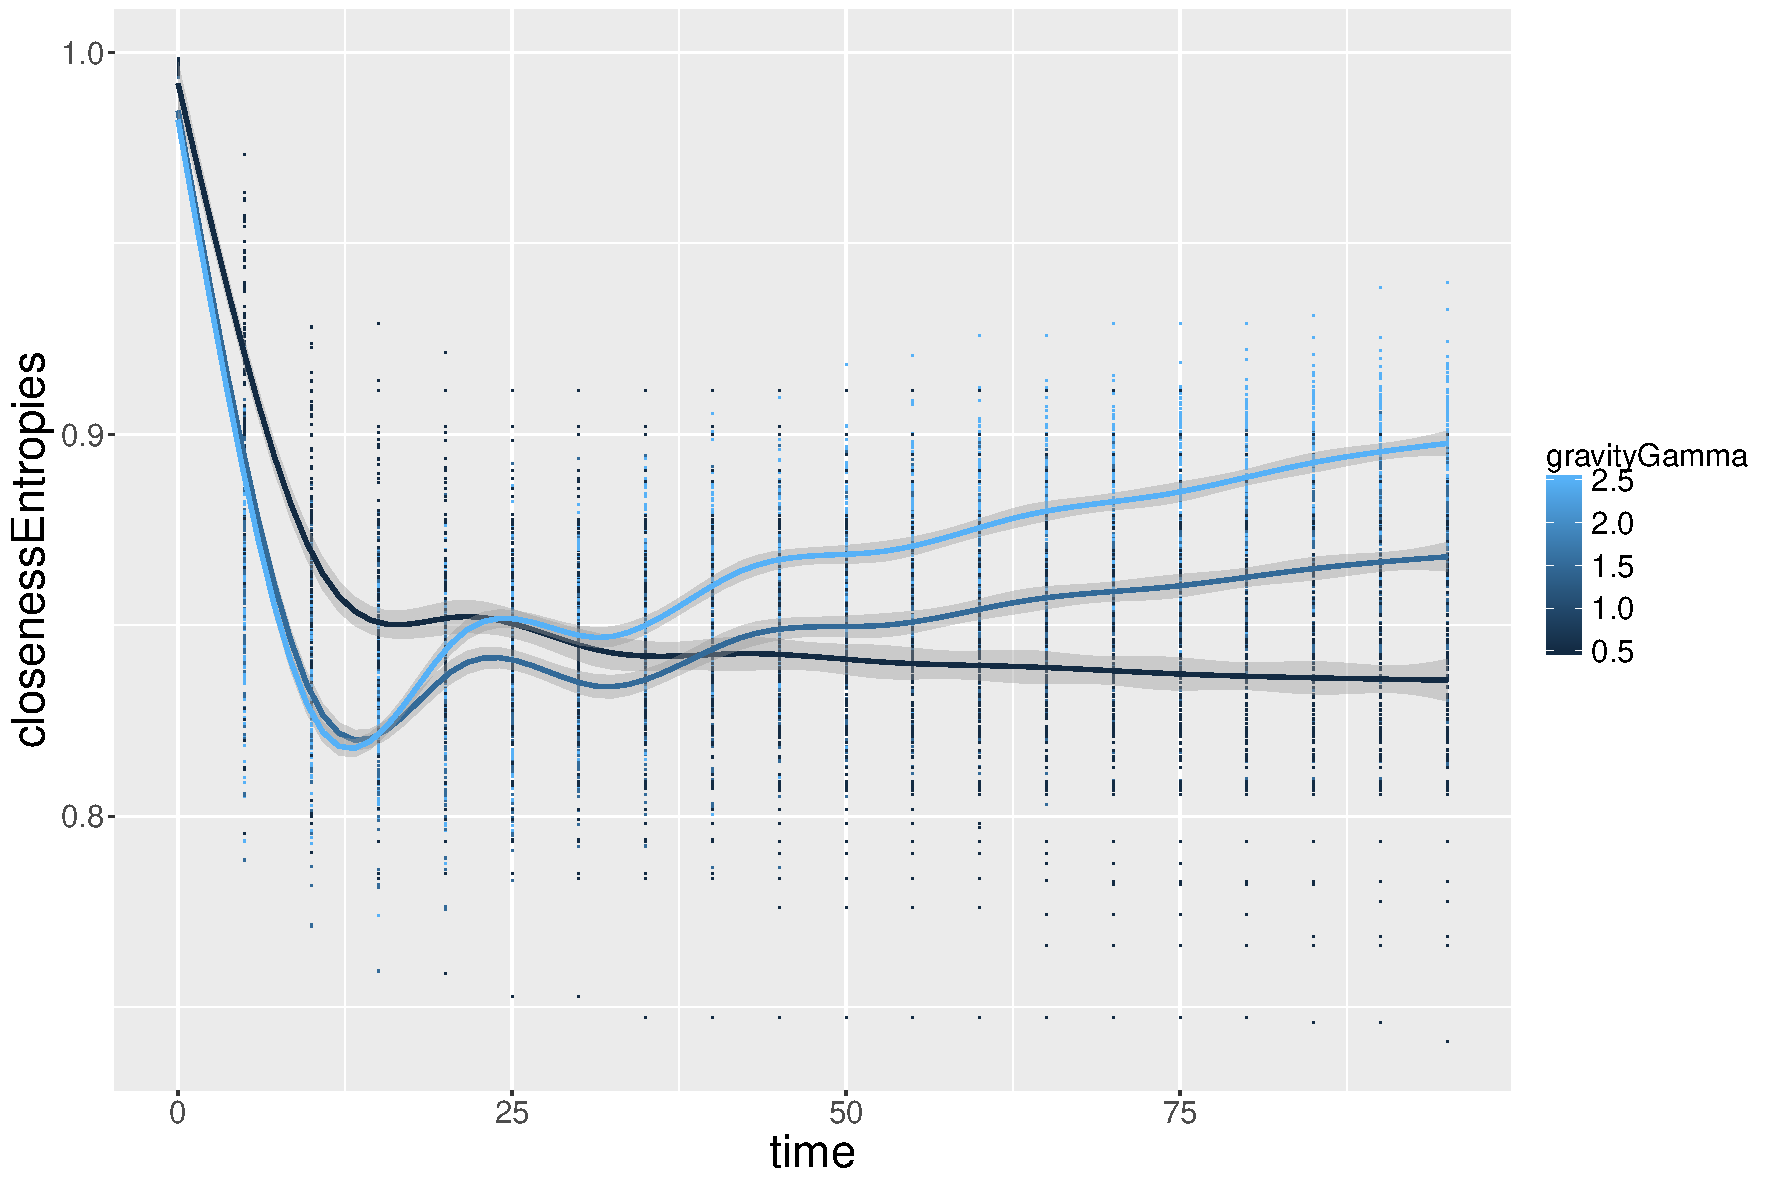
\includegraphics[width=0.48\linewidth]{Figures/MacroCoEvolExplo/closenessEntropies_networkGamma2.5_networkSpeed110_gravityDecay0.016_networkThreshold11.pdf}
	%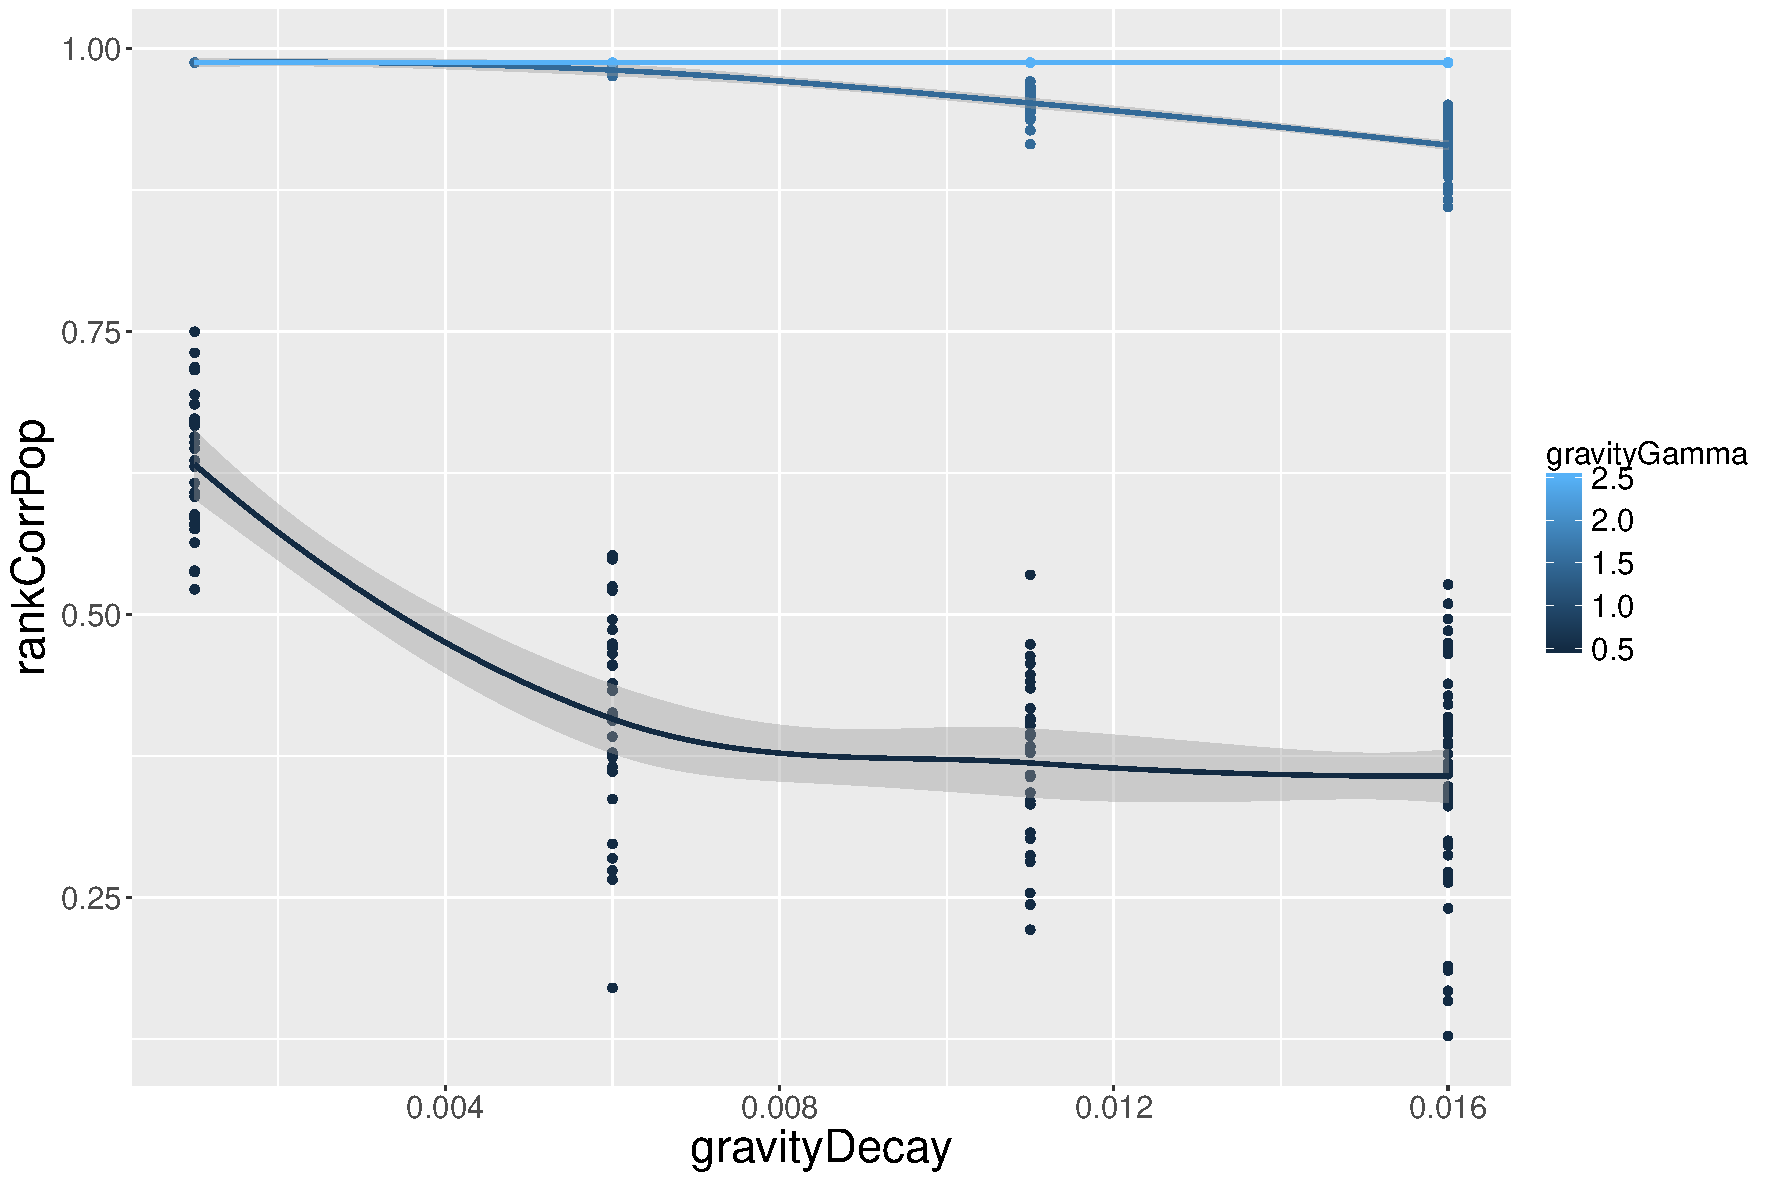
\includegraphics[width=0.48\linewidth]{Figures/MacroCoEvolExplo/rankCorrPop_networkSpeed110_networkThreshold11_networkGamma2.5.pdf}\\
	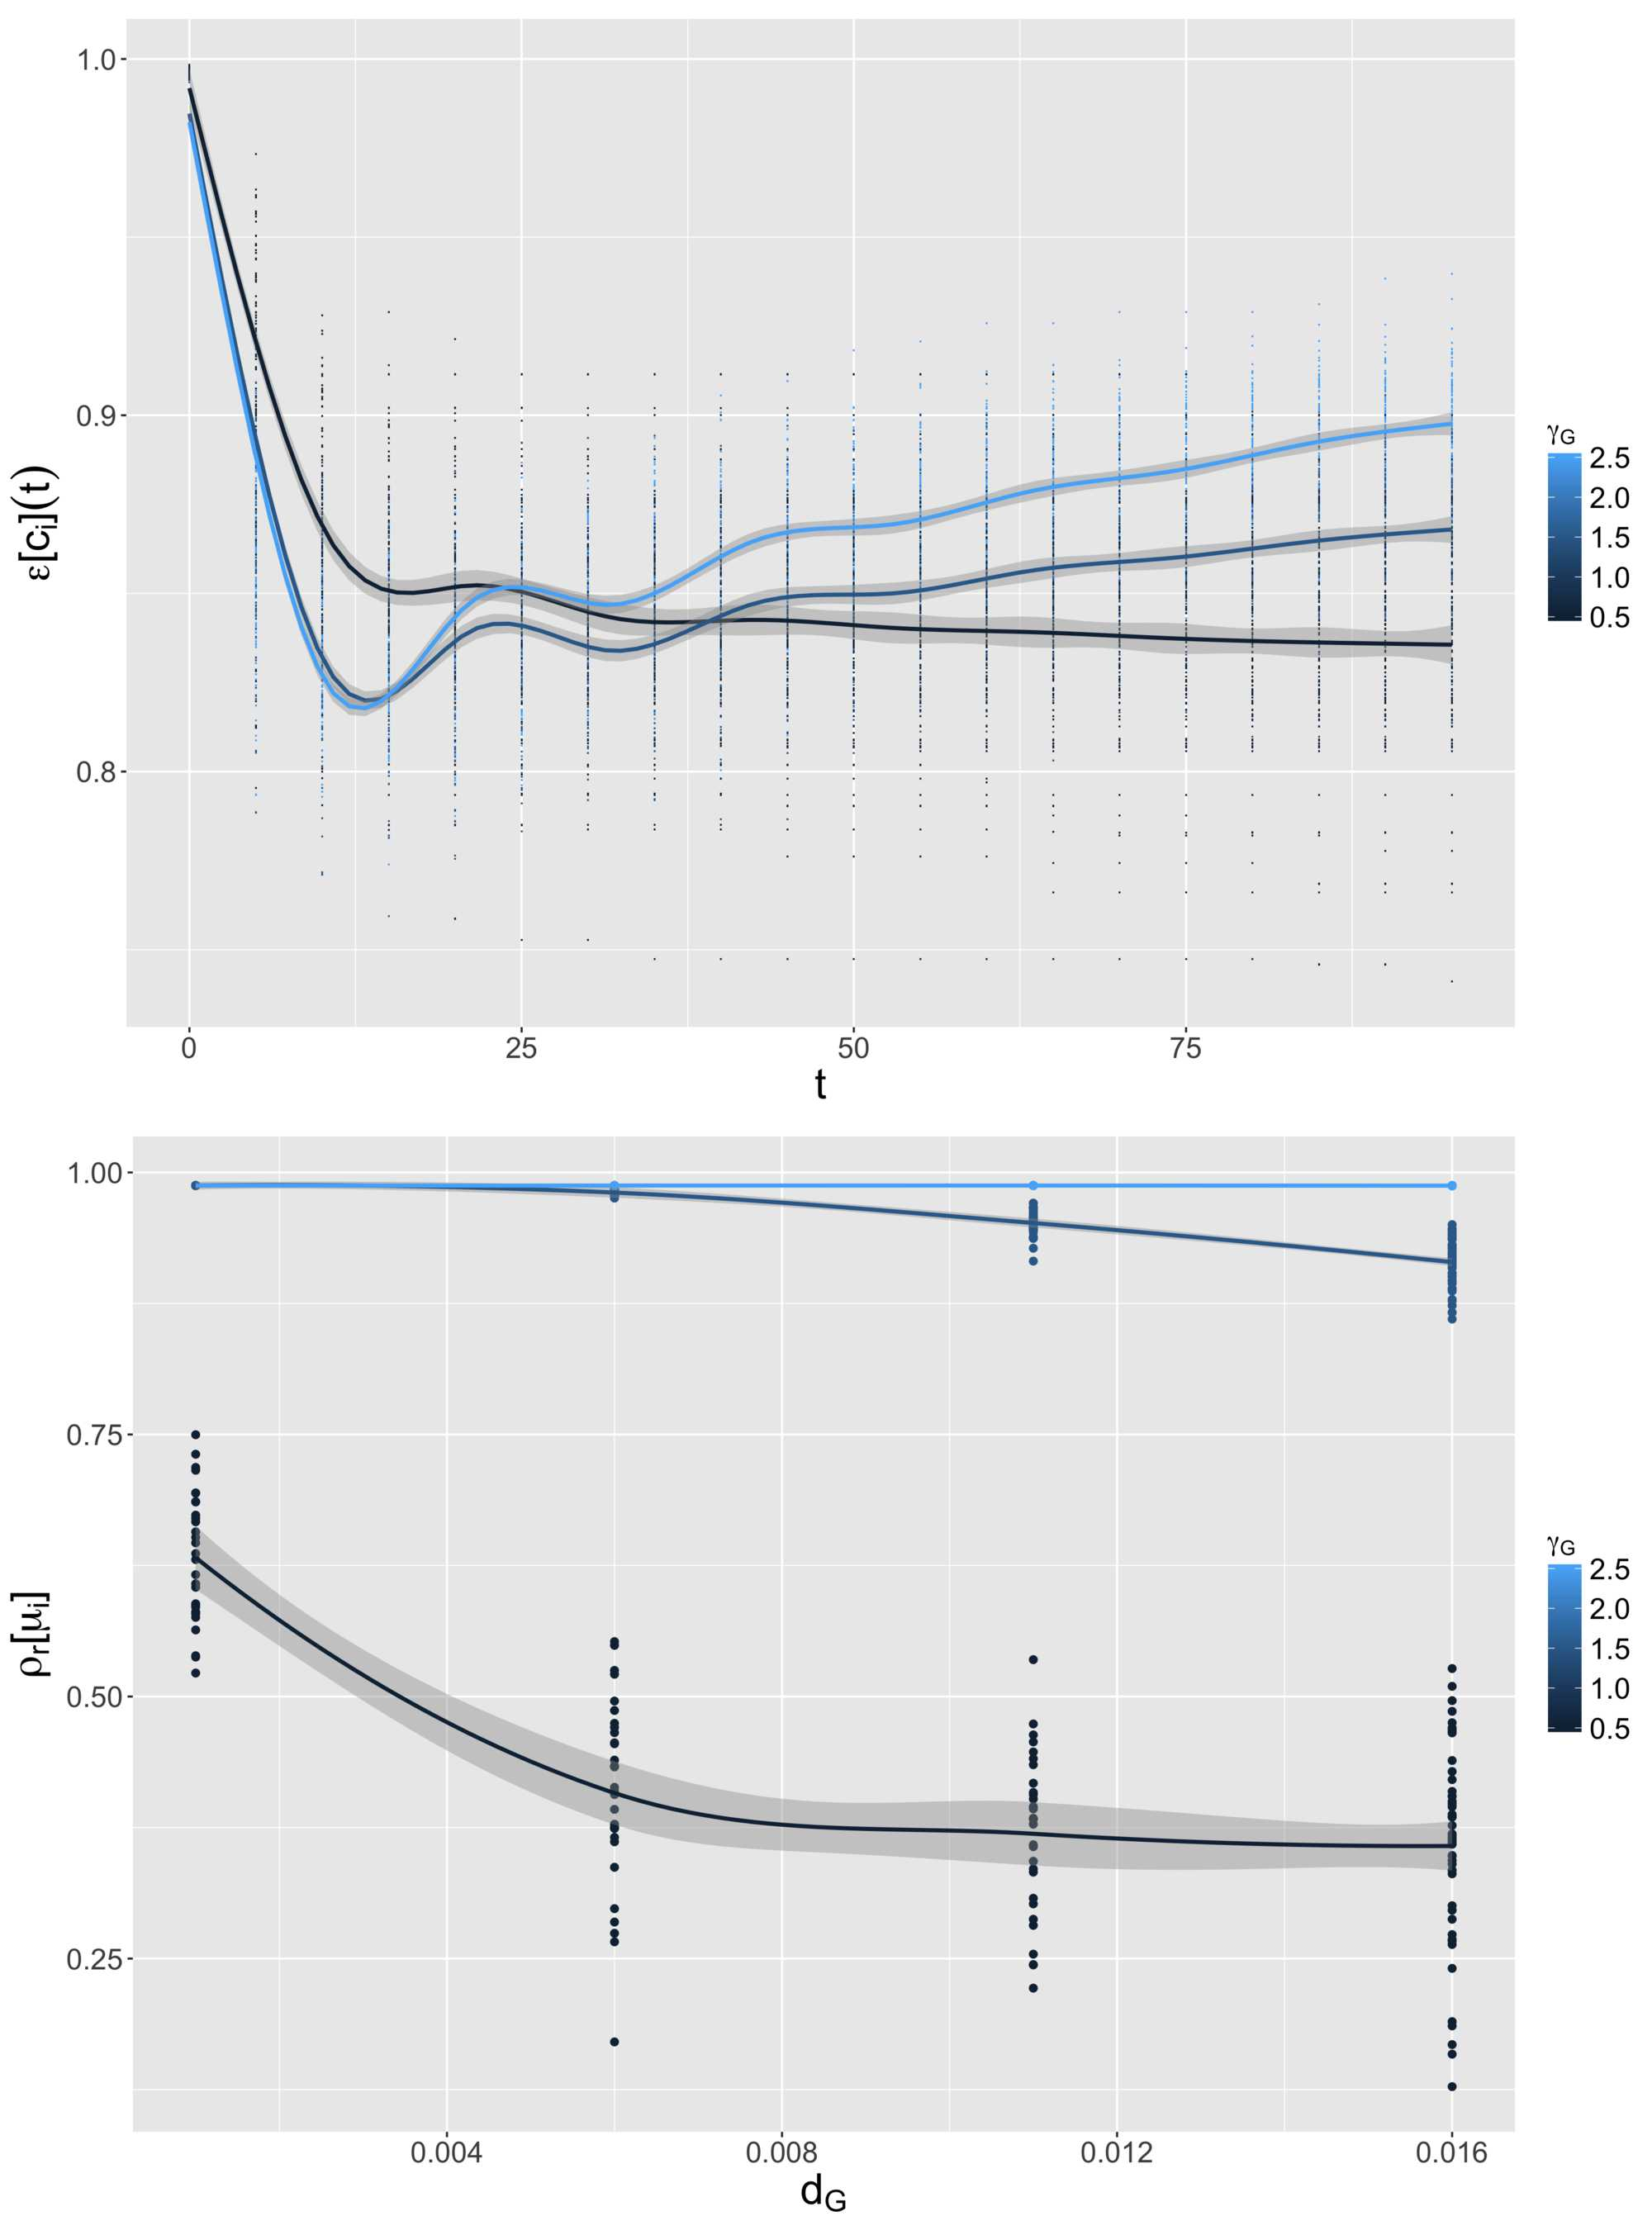
\includegraphics[width=\linewidth,height=0.85\textheight]{Figures/Final/6-1-3-fig-macrocoevolexplo-behavior.jpg}
	\caption[Behavior of the SimpopNet model][Comportement du modèle SimpopNet]{\textbf{Model behavior for the spatial configuration $N_S=80,\alpha_S=0.5,d_S=10,n_S=30$.} (\textit{Top}) Temporal trajectories of the entropy for closeness centralities, for $\gamma_N = 2.5$, $v_0 = 110$, $d_G = 0.016$, $\theta_N = 11$, as a function of $\gamma_G$ (color); (\textit{Bottom}) Rank correlation for population, as a function of $d_G$ and of $\gamma_G$ (color), for $\theta_N = 11$, $\gamma_N = 2.5$.\label{fig:macrocoevolexplo:behavior}}{\textbf{Comportement du modèle pour la configuration spatiale $N_S=80,\alpha_S=0.5,d_S=10,n_S=30$.} (\textit{Haut}) Trajectoires temporelles de l'entropie des centralités de proximité, pour $\gamma_N = 2.5$, $v_0 = 110$, $d_G = 0.016$, $\theta_N = 11$, en fonction de $\gamma_G$ (couleur); (\textit{Bas}) Corrélation de rang pour la population, en fonction de $d_G$ et de $\gamma_G$ (couleur), pour $\theta_N = 11$, $\gamma_N = 2.5$.\label{fig:macrocoevolexplo:behavior}}
\end{figure}
%%%%%%%%%%%%%%%%



\bpar{
The behavior of correlation indicators is shown in Fig.~\ref{fig:macrocoevolexplo:correlations}. Concerning the effect of distance on correlations between variables, i.e. the evolution of $\rho_d$, it is interesting to note that an increase of $d_G$ systematically diminishes the levels of correlation, what corresponds to the complexification that we previously showed. As expected, $\rho_d\left[d\right]$ decreases as a function of distance, and exhibits non zero values for the correlation between population and centrality for a high hierarchy $\gamma_G$, what shows that simultaneous adaptation regimes are rare in this model.
}{
Le comportement des indicateurs de corrélation est montré en Fig.~\ref{fig:macrocoevolexplo:correlations}. Concernant l'effet de la distance sur les corrélations entre variables, c'est-à-dire l'évolution de $\rho_d$, il est intéressant de noter que l'augmentation de $d_G$ diminue systématiquement les niveaux de corrélation, ce qui correspond à la complexification mise en valeur précédemment. Comme attendu, $\rho_d\left[d\right]$ décroit en fonction de la distance, et montre des valeurs non nulles pour la corrélation entre population et centralité pour une forte hiérarchie $\gamma_G$, ce qui montre que les régimes d'adaptation simultanée sont rares dans ce modèle.
}


\subsubsection{Causality regimes}{Régimes de causalité}


\bpar{
Finally, by studying $\rho_{\tau}$ (Fig.~\ref{fig:macrocoevolexplo:correlations}, bottom panel), we observe that causality regimes in the sense of~\ref{sec:causalityregimes} are not very varied (as the Fig.~\ref{fig:app:macrocoevolexplo:laggedcorrs} in Appendix~\ref{app:sec:macrocoevolexplo} confirms it for a broader range of parameters). The population is systematically caused by the centrality, but there exists no regime in which we observe the contrary. This is a logic of an effect of reinforcement of hierarchy by centrality, but not a configuration with circular causalities, and thus not a co-evolution properly speaking as we defined in the statistical sense.
}{
Enfin, en étudiant $\rho_{\tau}$ (Fig.~\ref{fig:macrocoevolexplo:correlations}, panneau du bas), nous constatons que les régimes de causalité au sens de~\ref{sec:causalityregimes} ne sont pas très variés (comme le confirme la Fig.~\ref{fig:app:macrocoevolexplo:laggedcorrs} en Annexe~\ref{app:sec:macrocoevolexplo} pour une plage plus large de paramètres). La population est systématiquement causée par la centralité, mais il n'existe pas de régime où l'on observe le contraire. Il s'agit d'une logique d'effet de renforcement de la hiérarchie par la centralité, mais pas d'une configuration avec causalités circulaires, et donc pas d'une une co-évolution à proprement parler comme nous l'avons définie au sens statistique.
}



% -- positive only
%unique(signs$sign)
%[1] "00/00/00" "00/00/10" "01/00/10" "00/10/00" "01/00/00"


%  -- with negative --
% unique(signs$sign)
% [1] "-1-1/00/00"     "-1-1/00/-10"    "-1-1/00/10"     "-10/00/00"      "-10/00/10"      "01/00/10"      
% [7] "00/00/10"       "-11/00/10"      "-1-1/-10/-10"   "-1-1/-1-1/-10"  "-1-1/-10/-1-1"  "-1-1/-1-1/-1-1"
% [13] "-1-1/10/-10"    "-1-1/-1-1/00"   "00/00/00"       "0-1/00/00"      "01/00/00"       "-1-1/-10/00"   
% [19] "01/00/-10"      "-1-1/1-1/-10" 



%%%%%%%%%%%%%%%%
\begin{figure}
	%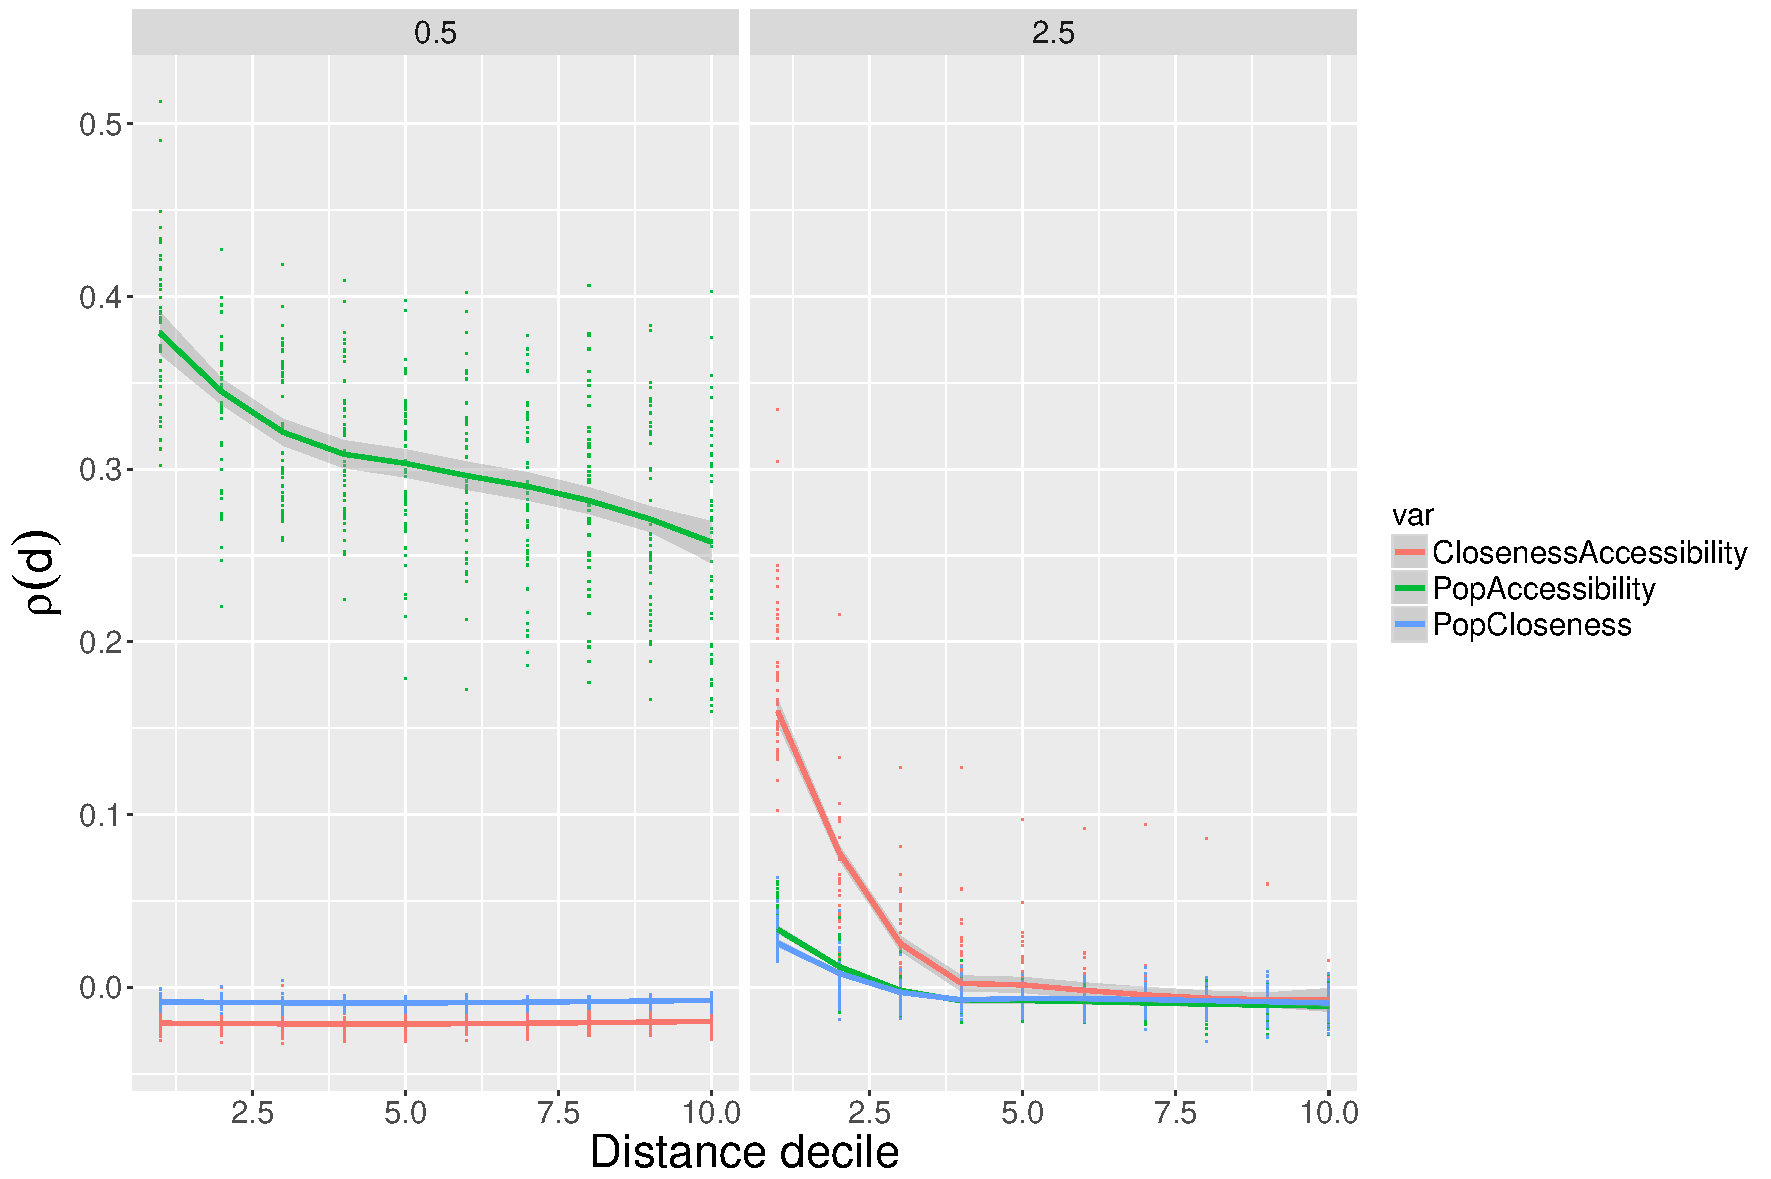
\includegraphics[width=0.48\linewidth]{Figures/MacroCoEvolExplo/distcorrs_networkGamma2.5_networkSpeed110_gravityDecay0.016_networkThreshold11.pdf}
	%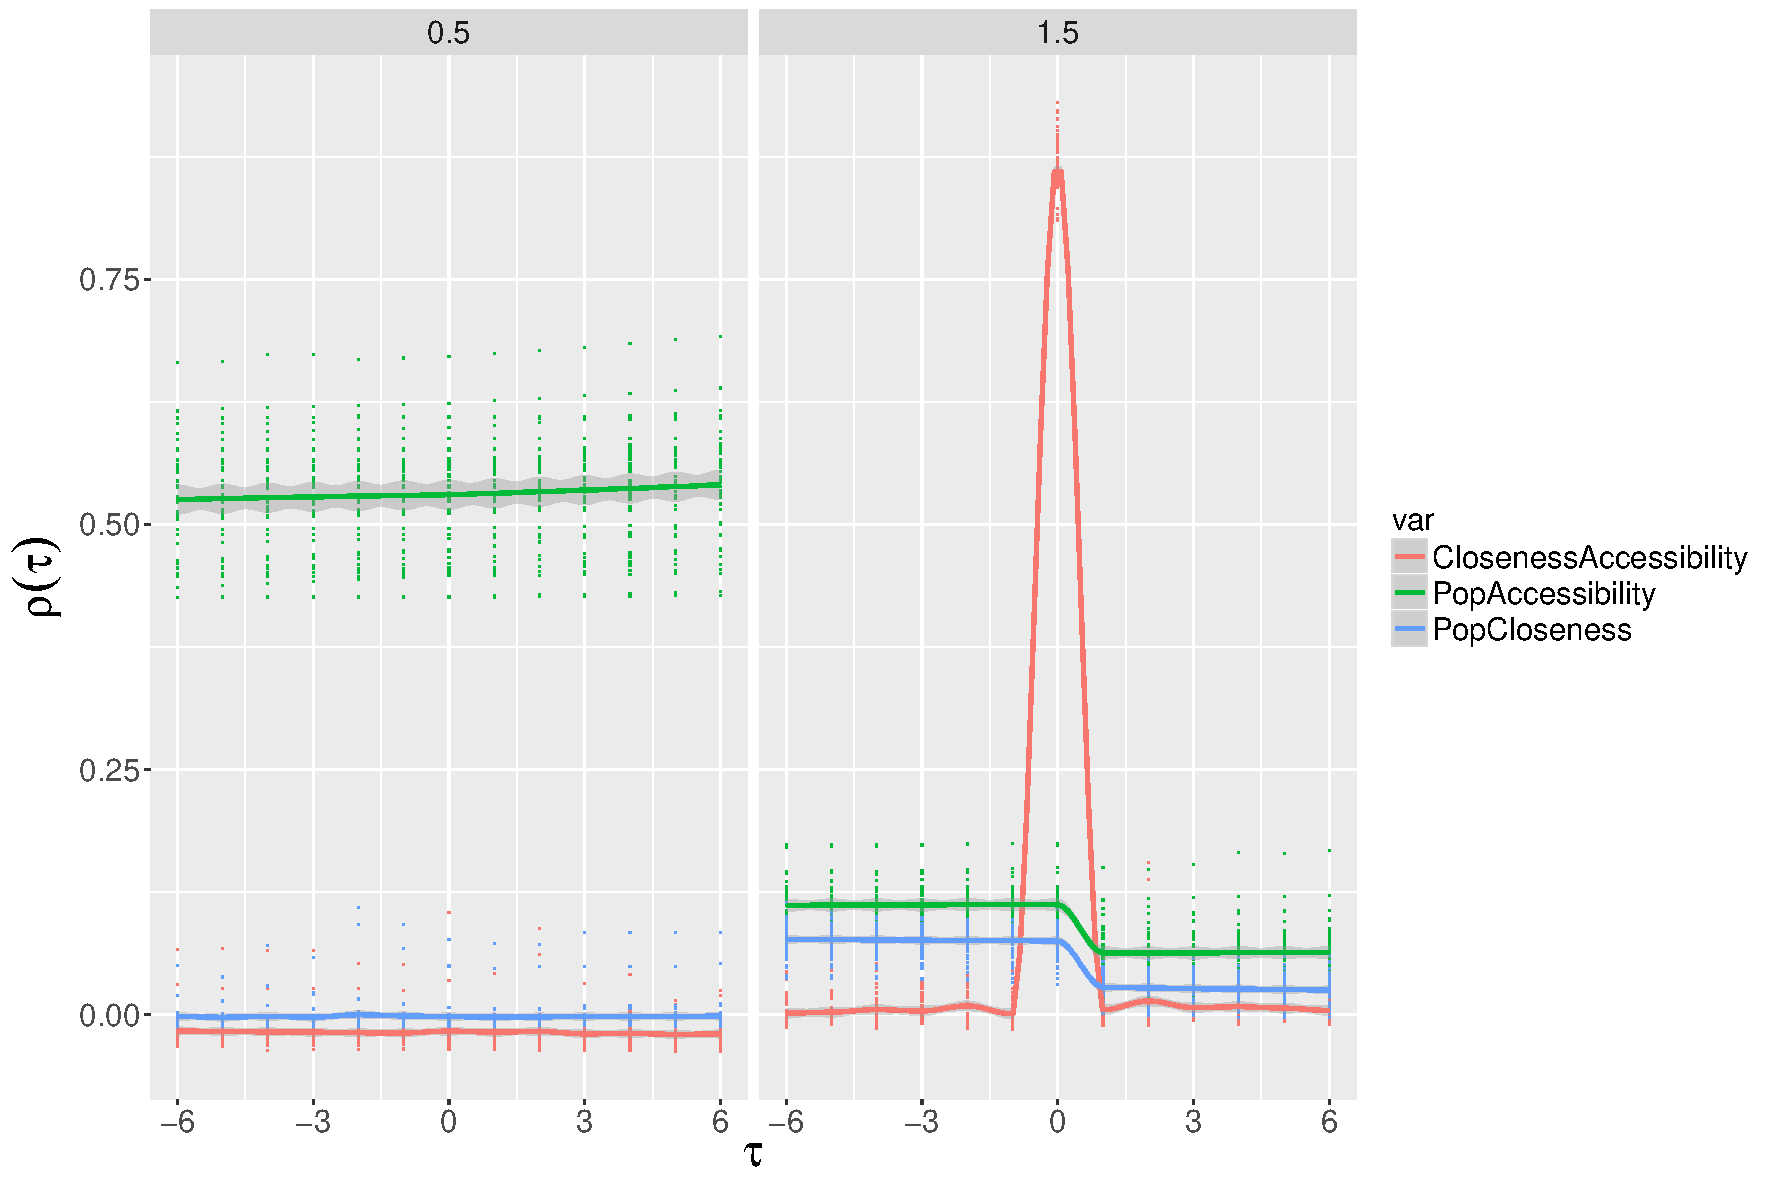
\includegraphics[width=0.48\linewidth]{Figures/MacroCoEvolExplo/laggedcorrs_networkGamma2.5_networkSpeed10_gravityDecay0.016_networkThreshold21.pdf}
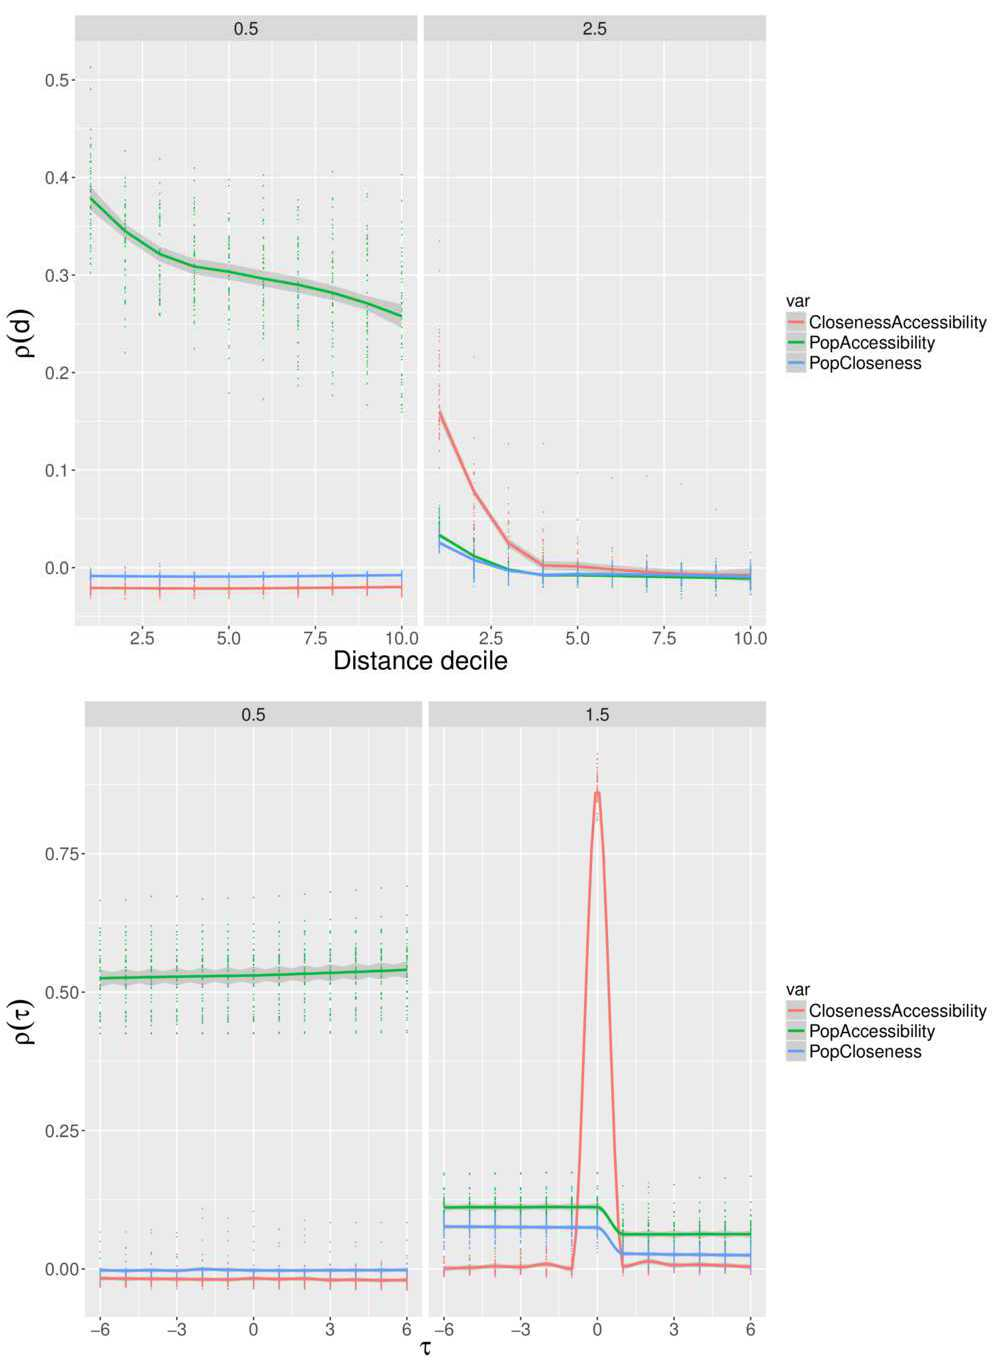
\includegraphics[width=\linewidth,height=0.9\textheight]{Figures/Final/6-1-3-fig-macrocoevolexplo-correlations.jpg}
	\caption[Correlations patterns in space and time][Motifs de corrélations dans l'espace et le temps]{\textbf{Correlations in the model for the spatial configuration $N_S=80,\alpha_S=0.5,d_S=10,n_S=30$.} (\textit{Top}) Correlations as a function of distance, for couples of variables (color), for $\gamma_N = 2.5$, $\theta_N = 21$, $v_0 = 10$, and for $d_G$ (columns) and $\gamma_G$ (rows) variables; (\textit{Bottom}) Lagged correlations for the same parameters. \label{fig:macrocoevolexplo:correlations}}{\textbf{Corrélations dans le modèle pour la configuration spatiale $N_S=80,\alpha_S=0.5,d_S=10,n_S=30$.} (\textit{Haut}) Corrélations en fonction de la distance, pour les couples de variables (couleur), pour $\gamma_N = 2.5$, $\theta_N = 21$, $v_0 = 10$, et pour $d_G$ (colonnes) et $\gamma_G$ (lignes) variables ; (\textit{Bas}) Corrélations retardées pour les mêmes paramètres.\label{fig:macrocoevolexplo:correlations}}
\end{figure}
%%%%%%%%%%%%%%%%


\bpar{
This brief exploration allows us to say that this model captures urban trajectories of a certain complexity, but that it does apparently not reproduces co-evolution regimes.
}{
Cette exploration brève nous permet d'affirmer que ce modèle capture des trajectoires urbaines d'une certaine complexité, mais qu'il ne reproduit apparemment pas de régimes de co-évolution.
}



\stars


\bpar{
We have thus in this section introduced the tools to understand trajectories produced by a co-evolution model, and tested these on the SimpopNet model.
}{
Nous avons ainsi dans cette section introduit les outils pour comprendre les trajectoires produites par un modèle de co-évolution, et testé ceux-ci sur le modèle SimpopNet.
}


\bpar{
In the following, we will explore in the same spirit a co-evolutive extension of the interaction model developed in~\ref{sec:interactiongibrat}, and will aim at establishing to what extent it is able to capture co-evolutive dynamics.
}{
Par la suite, nous explorerons dans le même esprit une extension co-évolutive du modèle d'interaction développé en~\ref{sec:interactiongibrat}, et chercherons à établir dans quelle mesure il est capable de capturer des dynamiques co-évolutives.
}


\stars








